%
%  Chris Thoma
%
\documentclass[12pt,fullpage]{article}
\usepackage{fullpage}
\usepackage{psfrag}                                          % LaTeX graphics tool
\usepackage{pslatex}                                         % avoids the default cmr font
\usepackage{graphicx}                                        % graphics package 
\usepackage{epsfig} 
\usepackage{hyperref}
\usepackage{color}

\begin{document}

\noindent
{\bf Log-Logistic distribution} (from \color{blue}\url{http://www.math.wm.edu/~leemis/chart/UDR/UDR.html}\color{black})

\noindent
The shorthand $X \sim {\rm loglogistic}(\lambda, \kappa)$ is used to indicate that the
random variable $X$ has the log-logistic distribution with positive scale parameter $\lambda$ and positive shape parameter $\kappa$.
A log-logistic random variable $X$ with parameters $\lambda$ and $\kappa$ 
has probability density function 
$$
f(x) = \frac{\lambda \kappa (\lambda \kern 0.08 em x)^{\kappa-1}}{(1 + (\lambda\kern 0.08 em  x)^\kappa)^2} \qquad \qquad x > 0
$$
for $\lambda > 0$, $\kappa > 0$.
The log logistic distribution can be used to model the lifetime of an object, the lifetime of a organism, or a service time.
The probability density function with three different parameter settings is illustrated below.
{\begin{figure}[h!]
\begin{center}
\psfrag{lab1}{$\lambda \kern -0.08 em = \kern -0.08 em 1, \kappa \kern -0.08 em = \kern -0.08 em 2$}
\psfrag{lab2}{$\lambda \kern -0.08 em = \kern -0.08 em 5, \kappa \kern -0.08 em = \kern -0.08 em 1$}
\psfrag{lab3}{$\lambda \kern -0.08 em = \kern -0.08 em 1, \kappa \kern -0.08 em = \kern -0.08 em 5$}
\psfrag{labx}{$x$}
\psfrag{labf}{$f(x)$}
\includegraphics[width=3.2in]{LoglogisticPlot.ps}
\end{center}
\end{figure}}\\
The cumulative distribution function on
the support of $X$ is 
$$
F(x) = P(X \le x) = \frac{(\lambda \kern 0.08 em x)^\kappa}{1+ (\lambda \kern 0.08 em x)^\kappa} \qquad \qquad x > 0.
$$
The survivor function on the support of $X$ is
$$
S(x) = P(X \ge x) =  \frac{1}{1+ (\lambda \kern 0.08 em x)^\kappa}\qquad \qquad x > 0.
$$
The hazard function on the support of $X$ is
$$
h(x) = \frac{f(x)}{S(x)} = \frac{\lambda \kappa(\lambda \kern 0.08 em x)^{\kappa-1}}{1 + (\lambda\kern 0.08 em x)^\kappa } \qquad \qquad x > 0.
$$
The cumulative hazard function on the support of $X$ is
$$
H(x) = -\ln(S(x)) = \ln[1+(\lambda \kern 0.08 em x)^\kappa] \qquad \qquad x > 0.
$$
The inverse distribution function of $X$ is
$$
F ^ {-1}(u) =  \frac{1}{\lambda} \left( \frac{u}{1-u} \right)^{1/\kappa} \qquad \qquad 0 < u < 1.
$$
The median of $X$ is
$$
\frac{1}{\lambda}.
$$
The moment generating function of $X$ is
$$
M(t) = E\left[ e ^ {\kern 0.04 em tX} \right] =  \displaystyle \int _{0}^{\infty } \frac{{e^{\kern 0.04 em tx}}{\lambda}^{\kappa}\kappa\,{x}^{\kappa-1}}{ \left( 1+(\lambda x)^\kappa \right)^2} dx
\qquad \qquad t > 0.
$$
The characteristic function of $X$ is
$$
\phi(t) = E\left[ e ^ {\kern 0.04 em itX} \right] = \displaystyle \int _{0}^{\infty } \frac{{e^{\kern 0.04 em itx}}{\lambda}^{\kappa}\kappa\,{x}^{\kappa-1}}{ \left(1+(\lambda x)^\kappa \right)^2} dx
\qquad \qquad t > 0.
$$
The population mean and variance are
$$
E[X] = \frac{\pi} {{\kappa}{\lambda} \left( \sin \left( {\frac {\pi }{\kappa}} \right)  \right)} \qquad \qquad 
V[X] = \frac{\pi \left( 2 \kappa \left(1 -\cos \left( {\frac {\pi }{\kappa}} \right)^2 \right) +\pi \sin \left( {\frac {\pi \, \left( \kappa+2 \right)}{\kappa}} \right) \right)} { \left( \sin \left( {\frac {\pi \left( \kappa+2 \right) }{\kappa}} \right)  \right) \left(  \left( \cos \left( {\frac {\pi }{\kappa}} \right)  \right)^2
\mbox{}-1 \right)(\lambda \kappa)^2} \qquad \qquad 
$$
%$$
%E\left[ \left( \frac{X - \mu}{\sigma} \right) ^  {\kern -0.04em 3} \right] = (\kappa \lambda)^3\left[- \frac{3\pi}{\lambda^3 \kappa \sin \left(\frac{\pi(\kappa +3)}{\kappa}\right)} + \frac{6\pi^2}{\kappa^2\lambda^3 \sin\left(\frac{\pi}{\kappa}\right)\sin \left( \frac {\pi\left( \kappa+2 \right)}{\kappa}\right)} + \frac{2\pi^3}{(\kappa \lambda)^3\sin\left(\frac{\pi}{\kappa}\right)^3}\right]-\frac{\sin \left( \frac {\pi\left( \kappa+2 \right)}{\kappa}\right)\left(1-\cos\left(\frac{\pi}{\kappa}\right)^2\right)}}{\pi \left[ 2 \kappa \left(1 -\cos \left( {\frac {\pi }{\kappa}} \right)^2 \right)+\pi \sin \left({\frac {\pi \, \left( \kappa+2 \right)}{\kappa}}\right)\right]}.
%$$

\noindent
{\bf APPL verification:}
The APPL statements
\begin{verbatim}
X := LogLogisticRV(lambda, kappa);
CDF(X);
SF(X);
HF(X);
CHF(X);
IDF(X);
MGF(X);
Mean(X);
Variance(X);
Skewness(X);
Kurtosis(X);
\end{verbatim}
verify the cumulative distribution function, survivor function, hazard function, cumulative hazard function, inverse, moment generating function, population mean, variance, skewness, and kurtosis.

\end{document}
